\documentclass[numerate]{cheatsheet}
\usepackage{bm}
\usepackage{textcomp, mathcomp}
\usepackage{empheq}
\usepackage{pbox}
\usepackage{booktabs}

\lstset{style=python_style}

\doctitle{Informatik 2 Cheatsheet}
\author{Julian Lotzer – jlotzer@student.ethz.ch\\ 
Daniel Steinhauser – dsteinhauser@student.ethz.ch\\
Modified by:
Christian Leser - cleser@ethz.ch
\\ \vspace*{-0.2em}}

\begin{document}
\section{General Python}
	\subsection{Reference Semantics and Aliasing}
Everything is a pointer: l1 and l2 point to the same adress
\lstinputlisting{src/1_general_python/code/1_pointer_example.py}

If a copy is needed, use:
\lstinputlisting{src/1_general_python/code/1_copy_example.py}
    \subsection{Data Types}
    Python dynamically types variables, which means that the variable type can change during the program's execution
    \lstinputlisting{src/1_general_python/code/2_data_types.py}
    To convert the data type:
    \lstinputlisting{src/1_general_python/code/2_type_conversion.py}
    \subsubsection{Type Hints}
    help make code more legible
    \lstinputlisting{src/1_general_python/code/2_1_type_hints.py}
    \subsection{Input and Output}
    {\centering\underline{\textbf{Output}} \par}
    \lstinputlisting{src/1_general_python/code/3_output.py}
    {\centering\underline{\textbf{Input}} \par}
    \lstinputlisting{src/1_general_python/code/3_input.py}
    \subsection{Control Flows (if/else, while, for)}
    {\centering\underline{\textbf{if, else}} \par}
    \lstinputlisting{src/1_general_python/code/4_if_else.py}

    {\centering\underline{\textbf{while}} \par}
    \lstinputlisting{src/1_general_python/code/4_while.py}

    {\centering\underline{\textbf{for with range}} \par}
    \lstinputlisting{src/1_general_python/code/4_for_list.py}

    {\centering\underline{\textbf{for with lists}} \par}
    \lstinputlisting{src/1_general_python/code/4_for_range.py}

    \subsection{Functions}
    Functions do not have to be declared in a specific order
    \subsubsection{Function Declaration}
    \lstinputlisting{src/1_general_python/code/5_1_declaration.py}
    \subsubsection{Default arguments}
    When calling a function with default arguments, it is not necessary to call the function with arguments.
    \lstinputlisting{src/1_general_python/code/5_2_default_args.py}
    \subsubsection{Global and local variables}
    {\centering\textcolor{red}{Avoid this kind of code!} \par}
    global variables can be used within a function if declared before the funciton call. Also, local variables can be made global:
    \lstinputlisting{src/1_general_python/code/5_3_global_local.py}

\section{Python Containers}
    \subsection{Operations on Containers}
    Number of Elements:
\begin{lstlisting}
len(c)
\end{lstlisting}
    Contains element x?
\begin{lstlisting}
x in c
\end{lstlisting}
Iterate over all elements:
\begin{lstlisting}
for x in c:
print(x)
\end{lstlisting}
    \subsection{Sequences (ordered containers)}
    \subsubsection{Sequence Operations (Überarbeiten)} \label{section_sequence_operations}
Subscript-Operator l[i]:
\begin{lstlisting}
l = [1, 3, 'hi', -4]
print(l[2]) #output: hi
\end{lstlisting}
Enumeration:
\lstinputlisting{src/3_containers/code/2_1_enumeration.py}
Combine sequences s1 and s2 (zip):
\lstinputlisting{src/3_containers/code/2_1_zip.py}
Output with a for loop:
\lstinputlisting{src/3_containers/code/2_1_loop_output.py}
Slicing (partial sequence) of a sequence s:
\lstinputlisting{src/3_containers/code/2_1_slicing.py}
    \subsubsection{List (mutable)}
{\centering\underline{\textbf{Initialise a list with []}} \par}
\begin{lstlisting}
l = [1, 3, "hi", -4]
M = [[-1 for i in range(n)] for j in range(m)]
# 2D list or m x n-Matrix filled with -1
\end{lstlisting}

{\centering\underline{\textbf{Common List Operations}} \par}
\lstinputlisting{src/2_containers/code/2_2_list_operation.py}

{\centering\underline{\textbf{List Comprehension}} \par}
Apply a function $f(x)$ to all items in list l:
\begin{lstlisting}
l2 = [f(x) for x in l] #z.g. 2*x for f(x)
\end{lstlisting}
Apply a function $f(x)$ to a range:
\begin{lstlisting}
r2 = [f(x) for x in range(1,6)]
\end{lstlisting}
Apply a function $f(x)$ only to items in list l that satisfy $g(x)$ (filter):
\begin{lstlisting}
l3 = [f(x) for x in l if g(x)]
\end{lstlisting}
Example: Read a sequence of numbers:
\begin{lstlisting}
l = [int(x) for x in input("Input: ").split()]
\end{lstlisting}
    \subsubsection{Tuple (immutable)}
{\centering\underline{\textbf{Initialise a tuple}} \par}
\begin{lstlisting}
t = ("a", 0, -6, 3.3)
\end{lstlisting}
    \subsubsection{Range (immutable)}
{\centering\underline{\textbf{Initialise a range}} \par}
\begin{lstlisting}
#range(start, stop, step)
#befault: start = 0, step = 1, end not included
r = range(0, 8, 2) #r ->  0   2   4   6,
\end{lstlisting}
    \subsubsection{String (immutable)}
{\centering\underline{\textbf{Initialise a string}} \par}
\begin{lstlisting}
s = "hello" #s ->  'h' 'e' 'l' 'l' 'o'
#you can use both " or ' for strings 
\end{lstlisting}

{\centering\underline{\textbf{Common String Operations}} \par}
\lstinputlisting{src/2_containers/code/2_5_str_operations.py}
Example: check if s is a string with content:
\begin{lstlisting}
type(s) == str and len(s.strip()) #False if empty
\end{lstlisting}
To convert a string s to a list of words:
\begin{lstlisting}
s.split(seperator, maxsplit) 
#seperator and maxsplit are optional
#s.split() -> split at all whitespaces
#separator = ", " -> split at every ", "
#maxsplit = 10 -> split only at first 10 separators
\end{lstlisting}
    \subsection{Collections (unordered containers)}
    \subsubsection{Set (non-associative)}
{\centering\underline{\textbf{Initialise Set}} \par}
\begin{lstlisting}
s = {1, 29, 12}
\end{lstlisting}

{\centering\underline{\textbf{Common Set Operations}} \par}
\lstinputlisting{src/3_containers/code/3_1_set_operations.py}
    \subsubsection{Dictionary (associative)}
See \ref{section_sequence_operations} Sequence operations for 'enumerate' and 'zip'\\
{\centering\underline{\textbf{Initialise a Dictionary with \{\}}} \par}
A dictionary consists of \textbf{tuples (key, value)} as items. For that reason, one can think of it as a list of tuples (Which it is not in reality)
\lstinputlisting{src/3_containers/code/3_2_initialise_dict.py}

{\centering\underline{\textbf{Common Dictionary Operations}} \par}
\lstinputlisting{src/3_containers/code/3_2_dict_operations.py}

{\centering\underline{\textbf{Iterate over a Dictionary}} \par}
\lstinputlisting{src/3_containers/code/3_2_iterate_over_dict.py}

{\centering\underline{\textbf{Dictionary Comprehension}} \par}
Transform a set into a dictionary by applying $f(x)$ and $g(x)$ on every element in the set:
\begin{lstlisting}
d3 = {f(x):g(x) for x in s} #s being a set
d4 = {f(x):g(y) for x, y in z.items()} #z being a dict
\end{lstlisting}
Transform a set into a dictionary, only if the element satisfies h(x):
\begin{lstlisting}
d5 = {f(x):g(x) for x in s if h(x)}
\end{lstlisting}
Example: Multiply the value of every odd key in a dictionary by 2:
\begin{lstlisting}
d6 = {k:2*v for k, v in d.items() if k % 2 == 1}
\end{lstlisting}

\section{Numpy}
    Pandas is a Python package which supports working with tabulated data.

To import pandas, use:
\begin{lstlisting}
import pandas as pd
\end{lstlisting}

Now you can refer to classes and functions from the package using ”pd”.
    \subsection{Python Lists vs. Numpy Arrays}
Numpy arrays are like Python lists. Below is a summary of the key differences.
\begin{tabular*}{\linewidth}{m{0.44\linewidth} | m{0.44\linewidth}}
    Python Lists & Numpy Arrays\\
    \hline
    Variable size & Fixed size\\
    \hline
    Different element types & Single element type\\
    \hline
    Mathematical operations on single elements only & Mathematical operations on whole arrays\\
    \hline
    Primarily 1D & Multi-dimensional\\
\end{tabular*}

    \subsection{Declaring Numpy Arrays}
{\centering\underline{\textbf{Using sequences}} \par}
\lstinputlisting{src/3_numpy/code/3_sequence.py}

{\centering\underline{\textbf{Using random numbers}} \par}
\lstinputlisting{src/3_numpy/code/3_random.py}

{\centering\underline{\textbf{Using arange command}} \par}
creates an array from the start to the stop value with a given step value, stop is \textbf{not} inclusive
\lstinputlisting{src/3_numpy/code/3_arange.py}

{\centering\underline{\textbf{Using linspace command}} \par}
creates a numpy array with num equally spaced elements between start and stop, stop is inclusive:
\lstinputlisting{src/3_numpy/code/3_linspace.py}
    \subsection{Numpy Array operations}
{\centering\underline{\textbf{Common numpy array operations}} \par}
• Return the number of elements:
a = np.arange(10)
a.size() #=10
• Accessing elements (1D array)
a[5] #=5
• Accessing elements (2D array):
A = np.array([[1,2,3],[4,5,6]])
A[1,2] #=A[1][2]=6
A[:,2] #array([3,6])
A[1,:] #array([4,5,6])

{\centering\underline{\textbf{Slicing}} \par}
• Slicing is dependent on the dimensions of the matrix. For 1D arrays:
A = np.arange(10) #[0,1,2,3,4,5,6,7,8,9]
A[2:5:2] #array([2,4])
• For 2D arrays (matrices):
A = np.array([[1,2,3],
	     [4,5,6],
              [7,8,9]])
A[0:2,1:3] #array([2,3],
                   [5,6])

{\centering\underline{\textbf{Statistics}} \par}
a = np.linspace(-4,-2,3) #array([-4,-3,-2])
• Minimum of all elements:
a.min() #-4 
• Maximum of all elements:
a.max() #-2
• Sum of all elements:
a.sum() #-9 
• Average of all elements:
np.mean(a) #-3
• Standard deviation of all elements:
np.std(a) #0.81 

{\centering\underline{\textbf{Mathematical Operations}} \par}
• Generally mathematical operations are carried out element-wise:
A = np.array([[2,3,4],[6,7,6]])
B = np.array([[1,9,1],[2,3,9]])
A+1
#array([[3,4,5],
       [7,8,7]])
A * 2 
#array([[4,6,8],
       [12,14,12]])
A ** 4 
#array([[16,81,256],
       [1296,2401,1296]])
np.sin(A) 
#array([[0.909,0.141,-0.756],
       [-0.279,0.657,-0.279]])
A + B 
#array([[3,12,5],
        [8,10,15]])
A * B 
#array([[2,27,4],
       [12.21,54]])
np.sum(A, axis = 0) 
#= A.sum(axis = 0) -> array([8,10,10])
np.sum(A, axis = 1) 
#= A.sum(axis = 1) -> array([9,19])

• Given that the dimensionality of two matrices is correct, one is able to multiply them using @:
A = np.array([[2,3,4],[6,7,6]])
A @ np.array([[1, 4], [3, 4], [4,6]]) 
#array([[27, 44], 
        [51, 88]])
• Using the dot() function to multiply two matrices:
A.dot(np.array([[1,4],[3,4],[4,6]]) 
#array([[27, 44], 
        [51, 88]])
• Using the dot() function to find the scalar product of two vectors:
a = np.array([1,2,3])
b = np.array([3,4,6])
a.dot(b) #29

{\centering\underline{\textbf{Filtering}} \par}
• Filter a numpy array using the subscript operator:
a = np.arange(7) #array([0,1,2,3,4,5,6])
f = a % 2 == 0
a[f] #array([0,2,4,6])

\section{Pandas}
    Pandas is a Python package which supports working with tabulated data.

To import pandas, use:
\begin{lstlisting}
import pandas as pd
\end{lstlisting}

Now you can refer to classes and functions from the package using ”pd”.
    \subsection{read CSV file into dataframe}
\begin{lstlisting}
climate = pd.read_csv("climate.csv", sep=",", index_col=0, usecols=["time", ...])
#"sep" -> what characters values in the csv file are separated by. "index_col" -> what the index column will be. "usecols" -> what columns of the csv data will be #selected.
\end{lstlisting}
    \subsection*{Pandas Dataframe operations}
A dataframe can be thought of as a 2D list (list within a list) supporting access in more semantic, meaningful ways compared to using indices. Visualized, a dataframe may look something like the following: 

{\centering
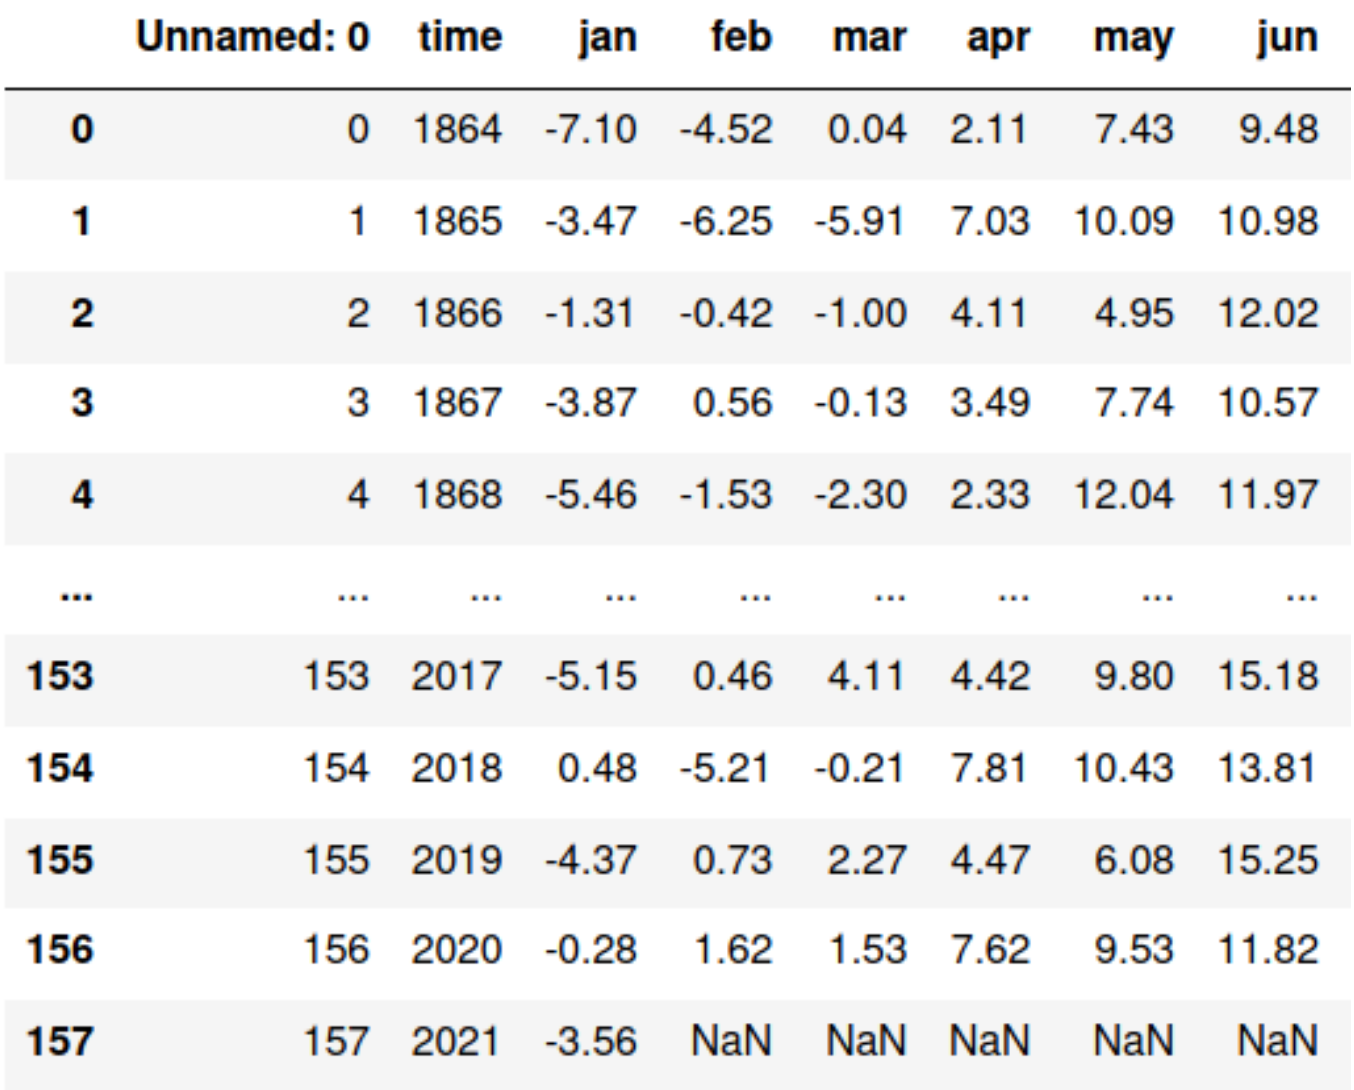
\includegraphics[width=0.8\linewidth]{src/4_pandas/images/pd_dataframe_index.png}\\
table of the climate, entries accessible via index \par}

The leftmost column is known as the "index column".  

{\centering\underline{\textbf{Change the Index Column}} \par}
\begin{lstlisting}
climate2 = climate.set_index("time") #creates copy
\end{lstlisting}
{\centering
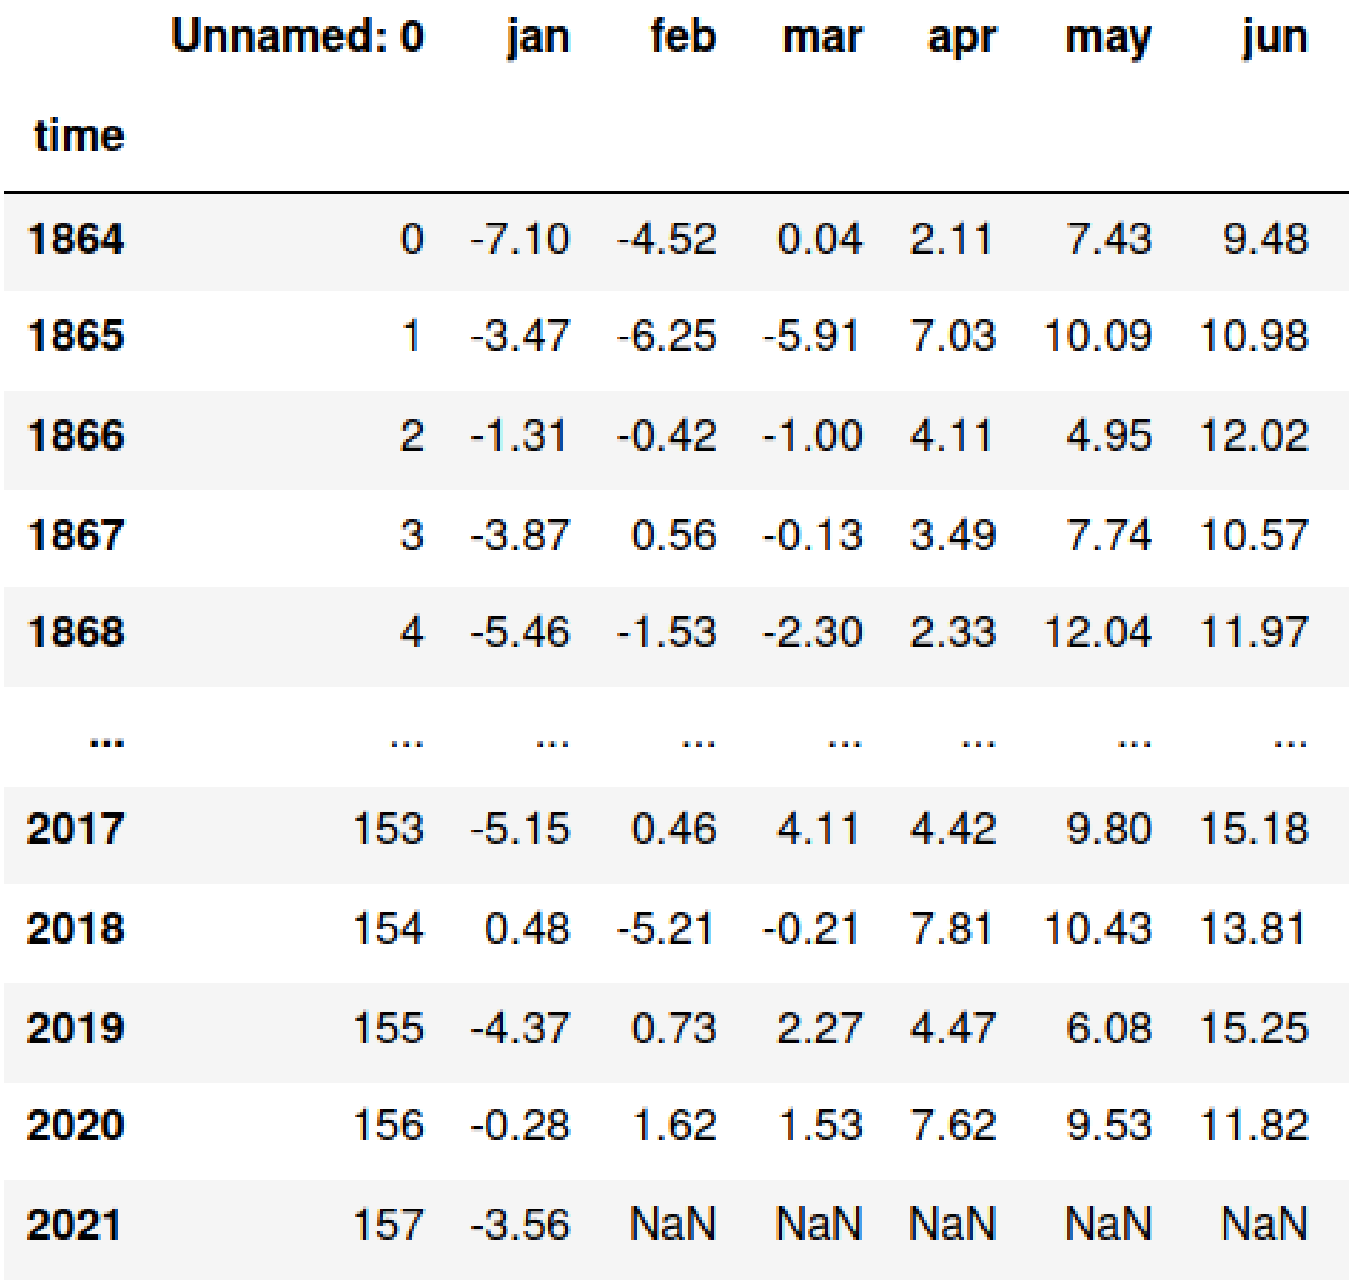
\includegraphics[width = 0.8\linewidth]{src/4_pandas/images/pd_dataframe_time.png}\\
table of the climate, entries accessible via time \par}

{\centering\underline{\textbf{Rename Columns}} \par}
\begin{lstlisting}
climate = climate.rename(columns={"old_index_name":"new_index_name", ...})
#renames the "old_index_name" column to "new_index_name"
\end{lstlisting}
rename all columns (len(data.columns) = number of colums must be true)
\begin{lstlisting}data.columns = ["Date", "January", "February", …]\end{lstlisting}

{\centering\underline{\textbf{Access Dataframe Elements}} \par}
Access a single column (type: Series):
\begin{lstlisting}
climate["feb"]
#gets the column "feb"
\end{lstlisting}
Access multiple columns (type: Dataframe):
\begin{lstlisting}
climate[["jan", "mar"]]
#gets the columns "jan" and "mar"
\end{lstlisting}
Access a single row, using an index (type: Series):
\begin{lstlisting}
climate.iloc[3]
#gets row 3
\end{lstlisting}
Multiple rows (type: Dataframe):
\begin{lstlisting}
Climate.iloc[1:4]
#gets rows 1 to 3
\end{lstlisting}
Access to a subtable using indices (type: Dataframe):
\begin{lstlisting}
climate.iloc[4:7,1:2]
#gets rows 4,7 with data only from column 1
\end{lstlisting}
Access to a subtable using index column values and column name (type: Dataframe):
\begin{lstlisting}
climate2 = climate.set_index("time")
climate2.loc[1864:1868,"jan":"mar"]
#includes the rows labeled with 1864 until and including #1868, the columns from "jan" until and including "mar"
\end{lstlisting}
Access to a single element:
\begin{lstlisting}
climate["jan"][3]
#gets the element in column "jan" in row 3
\end{lstlisting}

{\centering\underline{\textbf{Filter Dataframes}} \par}
Filter rows:
\begin{lstlisting}
climate[climate["jan"]>2]
#filters out the rows with values in the "jan" column #less than 2
\end{lstlisting}
• Example: All entries in "jan" with values more than 2:
\begin{lstlisting}
climate["jan"][climate["jan"]>2]
\end{lstlisting}

{\centering\underline{\textbf{Dealing with Invalid Data}} \par}
Convert all the values in a column to numeric:
\begin{lstlisting}
data[column] = pd.to_numeric(data[column], errors="coerce")
#converts all the values to numeric values. #errors="coerce" -> converts values which cannot be #converted to NaN.
\end{lstlisting}
Delete all rows containing NaN entries:
\begin{lstlisting}
data.dropna(axis = 0, how="any")
#how="any" -> delete row if any value is NaN.
#how="all" -> delete row if all values are NaN
#axis = 1 -> delete column instead of row
\end{lstlisting}
• Fill all entries containing NaN with a value:
\begin{lstlisting}
data.fillna(0) #fill any NaN entries with 0
\end{lstlisting}

{\centering\underline{\textbf{Modify Dataframes}} \par}
Add a column:
\begin{lstlisting}
climate["new_col"] = climate["time"] + climate["jan"] 
#"new_col" is a new column whose values are #those of the "time" and "jan" column added
\end{lstlisting}
Delete a column:
\begin{lstlisting}
climate = climate.drop(columns=["time"])
#delete the "time" column
\end{lstlisting}
Add a row:
\begin{lstlisting}
d = {"mar":34, "jan":23}
climate.append(d, ignore_index=True)
#adds another row with the values 34 for "mar" and 23 for #"jan". Other entries are NaN
\end{lstlisting}
Delete a row:
\begin{lstlisting}
climate = climate.drop(climate.index[0]) 
#deletes row 0
\end{lstlisting}
Transpose the dataframe:
\begin{lstlisting}
climate = climate.T
\end{lstlisting}

{\centering\underline{\textbf{Analyse Data}} \par}
Sum of all the entries in each column (type: Series):
\begin{lstlisting}
climate.sum()
\end{lstlisting}
Maximum of all the entries in each column (type: Series):
\begin{lstlisting}
climate.max()
\end{lstlisting}
Create a dataframe summarizing the max and sum for each column:
\begin{lstlisting}
climate.agg(["max","sum"])
#A dataframe containing the same columns as climate
#with row 0 containing the max of the column and row 1 #containing the sum of the column. The strings in the 
#list should be names of valid pandas Series functions. 
\end{lstlisting}
Get statistical information for each column (type: Dataframe):
\begin{lstlisting}
climate.describe()
#includes a variety of statistical measures
\end{lstlisting}
Sort a dataframe according to entries in a specific column(s):
\begin{lstlisting}
climate = climate.sort_values(["time", "jan"], ascending=False)
#sorts the rows by "time" in descending order. If two #entries for "time" are equal, then the rows are sorted #by "jan"
\end{lstlisting}
Split a dataframe into groups based on a specified column and perform a computation on each group:
\begin{lstlisting}
data.groupby("column").sum() 
#groups data based on the entries for "column" and #calculates the sum for each group.
data.groupby("column").max()
#groups data based on the entries for "column" and #calculates the max for each group.
\end{lstlisting}

\section{Matplotlib}
    Pandas is a Python package which supports working with tabulated data.

To import pandas, use:
\begin{lstlisting}
import pandas as pd
\end{lstlisting}

Now you can refer to classes and functions from the package using ”pd”.
    \subsection{Line and Scatter Plots}
To graph two numpy arrays, one representing the x values and the other representing the corresponding y values:
\begin{minipage}{0.49\linewidth}
    \lstinputlisting{src/5_matplotlib/code/2_line_scatter.py}
\end{minipage}
\begin{minipage}{0.49\linewidth}
    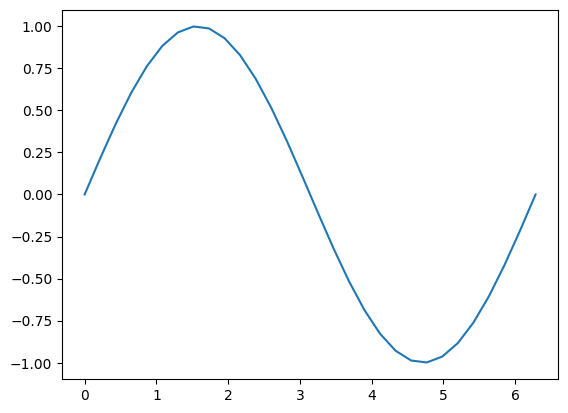
\includegraphics[width = \linewidth]{src/5_matplotlib/images/line_plot.png}
    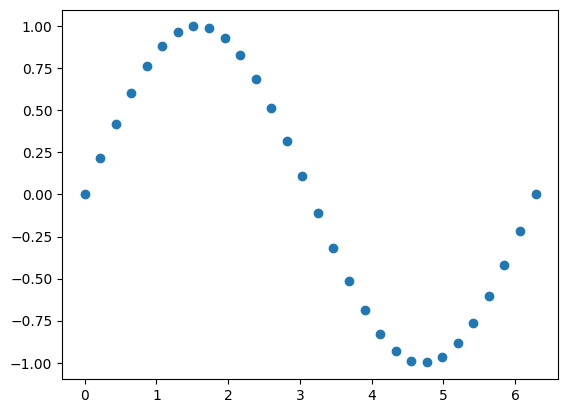
\includegraphics[width = \linewidth]{src/5_matplotlib/images/scatter_plot.png}
\end{minipage}

    \subsection{Histogram Plots}
To plot a histogram, use the following template:
\begin{minipage}{0.49\linewidth}
    \lstinputlisting{src/11_matplotlib/code/4_histogram.py}
\end{minipage}
\begin{minipage}{0.49\linewidth}
    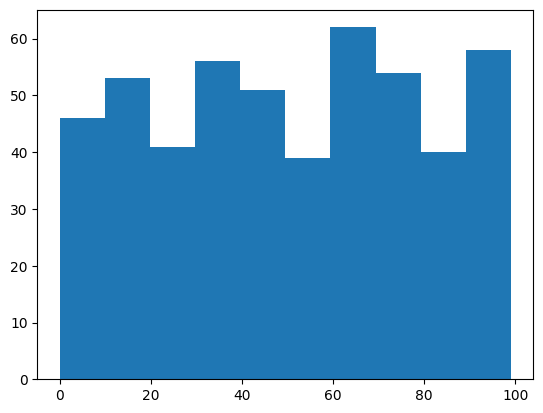
\includegraphics[width = \linewidth]{src/11_matplotlib/images/histogram_plot.png}
\end{minipage}


    \subsection{Graph Styling}
\lstinputlisting{src/5_matplotlib/code/5_styling.py}


\section{Algorithms}
    \subsection{Runtime analysis}
    \subsection{Invariants}
The invariant is a condition in an algorithm involving a loop.\\
\begin{tabular}{l | p{0.3\linewidth} | p{0.3\linewidth}}
    Phase & Description & Example (list 'a' is sorted until index 'i')\\
    \hline \hline
    1. Initialization & the condition is met before the loop & i = 0, a[:i] = a[0] \\
    \hline
    2. Continuation & the condition holds at each iteration & i = j, a[:j] \\
    \hline
    3. Termination & the condition holds at the end of the loop & i = n, a[:n] = a[n]
\end{tabular}
    \subsection{Sorting Algorithms}
    \subsubsection{Selection Sort}
        \begin{minipage}{0.59\linewidth}
            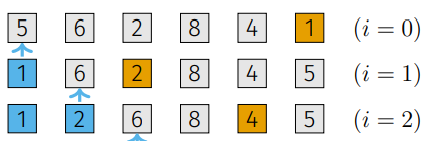
\includegraphics[width = \linewidth]{src/6_algorithms/images/selection_sort.png}
        \end{minipage}
        \begin{minipage}{0.39\linewidth}
            \fcolorbox{black}{cyan}{sorted list}\\
            \fcolorbox{black}{white}{unsorted list}\\
            \fcolorbox{black}{orange}{smallest value}
        \end{minipage}

        \lstinputlisting{src/6_algorithms/code/4_selection_sort.py}
        
        \begin{tabular*}{\linewidth}{| p{0.25\linewidth} | p{0.35\linewidth} | p{0.2\linewidth} |}
            \hline
            Case & Description & Runtime\\
            \hline \hline
            Worst-case & A is reverse sorted & $\Theta(n^2)$ \\
            \hline
            Average-case & - & $\Theta(n^2)$ \\
            \hline
            Best-case & A is already sorted & $\Theta(n)$ \\
            \hline
        \end{tabular*}
        
    \subsubsection{Insertion Sort}
        \begin{tabular*}{\linewidth}{| p{0.25\linewidth} | p{0.35\linewidth} | p{0.2\linewidth} |}
            \hline
            Case & Description & Runtime\\
            \hline \hline
            Worst-case &  &  \\
            \hline
            Average-case &  &  \\
            \hline
            Best-case &  &  \\
            \hline
        \end{tabular*}

    \subsubsection{Bubble Sort}
    \subsubsection{Mergesort (Divide and Conquer)}
    \subsubsection{Quick Sort (Divide and Conquer)}
    \subsection{Searching Algorithms}
    \subsubsection{Linear Search}
    \subsubsection{Binary Search}

\section{Data Structures}

\section{Programming Concepts}

\section{Dynamic Programming (DP)}

\section{Machine Learning (ML)}
\end{document}